% using pLaTeX
\documentclass[dvipdfmx, tikz, border=10pt]{standalone}
\usetikzlibrary{positioning, calc, intersections, arrows.meta}

\begin{document}

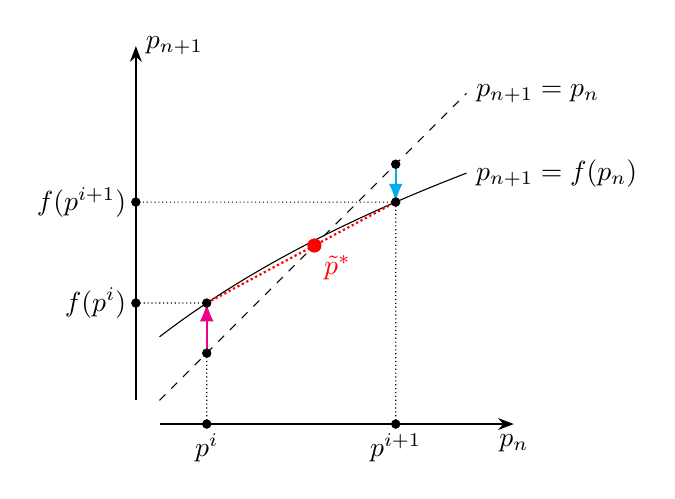
\begin{tikzpicture}[scale=3]
    \coordinate (O) at (0.2, 0.2); % origin
    % calculation points
    \foreach \x [count=\i] in {0.5, 1.3} % count starts from 1
        \coordinate (xp\i) at (\x, 0);

    \draw[-Stealth, semithick] ([xshift=0.1cm] O) -- ([xshift=1.6cm] O) node[below]{$p_n$}; % x軸
    \draw[-Stealth, semithick] ([yshift=0.1cm] O) -- ([yshift=1.6cm] O) node[right]{$p_{n + 1}$}; % y軸

    \draw[name path=line, domain=0.3:1.6, dashed] plot(\x, \x) node[right]{$p_{n + 1} = p_n$};
    \draw[name path=f, domain=0.3:1.6, samples=50] plot(\x, {ln((1 + \x) / 2) + 1}) node[right]{$p_{n + 1} = f(p_n)$};
    
    % (p^i, 0)
    \foreach \label [count=\i] in {i, i + 1} % count starts from 1
        \coordinate (p\i) at (O -| xp\i) node[below] at (p\i) {$p^{\label}$};

    % help lines
    \path[name path=vl1] (p1) -- ([yshift=1.5cm] p1);
    \path[name path=vl2] (p2) -- ([yshift=1.5cm] p2);
    % (p^i, p^i)
    \path[name intersections={of=vl1 and line, by={pp1}}];
    \path[name intersections={of=vl2 and line, by={pp2}}];
    % (p^i, f(p^i))
    \path[name intersections={of=vl1 and f, by={fp1}}];
    \path[name intersections={of=vl2 and f, by={fp2}}];
    % (0, f(p^i))
    \foreach \label [count=\i] in {i, i + 1}
        \coordinate (yfp\i) at (O |- fp\i) node[left] at (yfp\i) {$f(p^{\label})$};
    % lines
    \draw[densely dotted] (fp1) -- (yfp1);
    \draw[densely dotted] (fp2) -- (yfp2);
    \draw[densely dotted] (p1) -- (pp1);
    \draw[densely dotted] (p2) -- (fp2);

    \draw[-Latex, magenta, thick] (pp1) -- (fp1);
    \draw[-Latex, cyan, thick] (pp2) -- (fp2);

    % approximate fixed point
    \draw[name path=approx, thick, densely dotted, red] (fp1) -- (fp2);
    \path[name intersections={of=approx and line, by={pstar}}];

    % fill points
    \foreach \P in {p1, p2} \fill (\P) circle (0.2mm);
    \foreach \i in {1, 2} \fill (fp\i) circle (0.2mm) (pp\i) circle (0.2mm) (yfp\i) circle (0.2mm);
    \fill[red] (pstar) circle (0.3mm) node [below right] {$\tilde{p}^*$};
\end{tikzpicture}

\end{document}